\chapter{Marco teórico}

\section{Energía}
Seguramente el concepto de energía sea el más usado, conocido e importante en ciencias. A pesar de su gran empleo en la actualidad, fue desarrollado con lentitud a lo largo de los siglos y culminó con la ley de la conservación de la energía. Una de las diferentes formas de definir la energía es la siguiente: \textbf{La energía es la capacidad para realizar un trabajo}\cite{Atkins2014}. Por lo tanto, existe una gran cantidad de manifestaciones de la energía, y el calor es, quizá, la manifestación de energía más común. Es importante recordar que el calor no se considera como algo almacenado dentro de un cuerpo. Al igual que el trabajo, existe sólo como energía transitoria que va de un cuerpo a otro o entre un sistema y su medio. En termodinámica, existen varias cantidades que están relacionadas con la energía, entre ellas se encuentran la energía interna y la entalpía. Podemos definir a la \textbf{energía interna} como la suma de todas las energías cinéticas y potenciales de los componentes de un sistema (una definición muy conveniente para una escala macroscópica). No obstante, si nos refiriéramos a una escala microscópica, podríamos decir que, la energía interna es la energía relacionada con el movimiento aleatorio y desordenado de las moléculas, es decir, la energía interna esta formada por energías de traslación, rotación, vibración, electrónica y nuclear, así como interacciones intermoleculares. \\
\newpage
El símbolo que representa a la energía interna  es la letra \textit{\textbf{U}} y para cambios se expresa como: 

\begin{equation}
\Delta U = U_{2} - U_{1}
\label{eq:3.1}
\end{equation}

donde $U_{2}$ y $U_{1}$ son las energías internas del sistema en su estado final e inicial, respectivamente \cite{Chang2008}. El estudio de la variación de la energía interna en las transformaciones químicas es importante para el desarrollo de las bases teóricas de la química. Además, la variación de la energía interna es una magnitud indispensable para los cálculos termodinámicos de las reacciones químicas, porque tiene un gran significado para las investigaciones científicas y la industria. En el proceso de transformación de una sustancia, la energía interna se produce, como en otros casos, mediante la absorción o desprendimiento de calor y/o la realización de trabajo. El calor de una reacción química frecuentemente es apreciable; éste puede medirse directamente en muchos casos y es, precisamente, el objetivo de la \textbf{Termoquímica} estudiar el calor de las reacciones químicas \cite{Guerasimov1971}.\\


A la cantidad de energía de un sistema que se encuentra a presión constante se le conoce como \textbf{entalpía \textit{(H)}} y matemáticamente se define como 
\begin{equation}
 H = U + pV
 \label{eq:3.2}
\end{equation}
donde $U,$ $p$ y $V$ son  la energía interna, la presión y volumen del sistema. $H$ tiene unidades de energía, es decir: el \textbf{joule (J)}. Dado que $U,$ $p$ y $V$ son funciones de estado,  $H$ también lo será. Por lo tanto, el cambio en la entalpía dependerá sólo de las condiciones iniciales y finales del sistema:

\begin{equation}
\Delta H = H_{2} - H_{1} = (U_{2} + p_{2}V_{2})-(U_{1} + p_{1}V_{1})
\label{eq:3.3}
\end{equation}

\newpage
\section{Entalpía de reacción}

Existen procesos químicos que se llevan a cabo a presión constante, un ejemplo de ello son las reacciones químicas que pueden considerarse como sistemas termodinámicos. El cambio de entalpía que acompaña a una reacción se conoce como \textbf{entalpía de reacción} o \textbf{calor de reacción} y se representa como $\Delta_{\mathrm{r}}H$ \cite{Atkins2014}. Como cualquier sistema, el cambio en la entalpía puede ser exotérmico o endotérmico. Dicho lo anterior, en una reacción, se puede escribir el cambio en la entalpía como

\begin{equation}
	\Delta _\mathrm{r}H = H_{\mathrm{productos}} - H_{\mathrm{reactivos}}
\label{eq:3.4}
\end{equation}

\section{Calorimetría}

Es posible determinar en forma experimental el valor de $\Delta _\mathrm{r}H$. A este conjunto de técnicas se le conoce como \textbf{calorimetría}; el calorímetro es un dispositivo utilizado para medir el flujo de calor. Las técnicas y el equipo usado en calorimetría dependen de la naturaleza del proceso en estudio. Para muchas reacciones, como las que ocurren en disolución, es fácil controlar la presión y medir directamente el $\Delta H$.

\section{Entalpía de formación estándar}

Un proceso particularmente importante, que es usado para tabular datos termoquímicos, es la formación de un compuesto a partir de sus elementos que lo conforman. Al cambio de entalpía asociado con este proceso se le conoce como \textbf{entalpía de formación}, $\Delta_{\mathrm{f}}H$, donde el subíndice ``f'' indica que la sustancia se formó a partir de sus elementos químicos. Sus unidades son  kJ mol$^{-1}$. La magnitud de cualquier cambio de entalpía depende de la temperatura, la presión y el estado de agregación en el que se encuentren los reactivos y productos. Para comparar las entalpías de diferentes reacciones, debe definirse un conjunto de condiciones, conocido como \textbf{estado estándar}, en el que se tabulan la mayoría de las entalpías. \\El estado estándar de una sustancia es su forma pura a $p$ = 1 bar y una temperatura de interés, que generalmente se elige como $T$ = 298 K. El \textbf{cambio de entalpía estándar} de una reacción se define como el cambio de entalpía cuando todos los reactivos y productos se encuentran en sus estados estándar. El cambio de entalpía estándar se denota como $\enthalpy*{}$. \\
La \textbf{entalpía estándar de formación} de un compuesto, $\enthalpy*(f){}$, es el cambio de entalpía de una reacción que forma un mol del compuesto a partir de sus elementos, con todas las sustancias en sus estados estándar:

\begin{center}
elementos (en estado estándar) $\longrightarrow$ compuesto (1 mol en estado estándar)
\end{center}

Por lo regular, se reportan valor de $\enthalpy*(f){}$ a $T$ = 298 K. Si un elemento existe en más de una forma en condiciones estándar, la forma más estable del elemento es la que normalmente se utilizar para la reacción de formación, por ejemplo:

\begin{equation}
	2\mathrm{C(grafito){(s)}} + 3\mathrm{{H}_{2}(g)} + \frac{1}{2}\mathrm{{O}_{2}(g)} \longrightarrow \mathrm{C_{2}H_{5}OH}{\mathrm{(l)}}
\label{eq:3.5}
\end{equation}

La fuente elemental de oxígeno es $\ch{O2\gas}$, no $\ch{O\gas}$ ni $\ch{O3\gas}$, porque el $\ch{O2\gas}$ es la forma estable del oxígeno a \textit{T} = 298 K y $p$ = 1 bar. De forma similar, la fuente elemental del carbono es el grafito(s) y no el diamante(s), porque el grafito(s) es la forma más estable a \textit{T} = 298 K y \textit{p} = 1 bar. De igual manera, la forma más estable del hidrógeno en condiciones estándar es el $\ch{H2\gas}$, así que este se utiliza como la fuente del hidrógeno en la ecuación \ref{eq:3.5}.


Por convención, la entalpía estándar de formación de cualquier elemento es cero, porque no se necesita una reacción de formación cuando el elemento ya se encuentra en su estado estándar. Así, los valores de $\enthalpy*(f){}$ para el $\ch{C\sld}, \ch{H2\gas}, \ch{O2\gas}$ y los estados estándar de otros elementos son cero \cite{Chang2008}.

\begin{equation}
	\enthalpy*(f){} \ch{(grafito)\sld} = 0
\label{eq:3.6}
\end{equation}

\begin{equation}
	\enthalpy*(f){} \ch{(H2)\gas} = 0
\label{eq:3.7}
\end{equation}

\begin{equation}
	\enthalpy*(f){} \ch{(O2)\gas} = 0
\label{eq:3.8}
\end{equation}

Como se mencionó antes, no podemos determinar el valor absoluto de la entalpía de una sustancia. Sólo se pueden calcular valores relativos a una referencia arbitraria. En termodinámica, lo que nos interesa son los cambios de $H$, aunque todo valor de $\enthalpy*(f){}$ asignado arbitrariamente a un elemento funcionaría; con ceros los cálculos se simplifican \cite{Chang2008}. Los valores de $\enthalpy*(f){}$ pueden obtenerse con un método directo o indirecto, los cuales se describen a continuación.

\textbf{Método directo}. Este método funciona en compuestos que se pueden sintetizar con facilidad a partir de sus elementos. Por ejemplo, la formación de $\ch{CO2}\gas$ a partir de $\ch{C}\sld$ y $\ch{O2}\gas$.

\textbf{Método indirecto}. La mayor parte de los compuestos no se pueden sintetizar directamente a partir de sus elementos. En algunos casos, las reacciones suceden con demasiada lentitud o no llegan a concretarse. Por lo tanto, el valor de $\enthalpy*(f){}$ se puede determinar mediante la ley de Hess \cite{Chang2008}. 

\section{Ley de Hess} \label{sec:Hess}

Con frecuencia, el $\Delta_{\mathrm{r}}H$ de una reacción se calcula a partir de los valores tabulados de otras reacciones. Por ello, no es necesario realizar mediciones calorimétricas para todos las compuestos. Como la entalpía es una función de estado, el cambio de entalpía asociado con cualquier proceso químico sólo depende de la cantidad de materia que experimenta el cambio, y de la naturaleza del estado inicial de los reactivos y del estado final de los productos. Esto significa que si una reacción se lleva a cabo en una o en varias etapas, la suma de los cambios de entalpía asociados con las etapas individuales debe ser igual al cambio de entalpía asociado con el proceso de una sola etapa.\\

\newpage

La \textbf{ley de Hess} establece que si una reacción se realiza en una serie de etapas, el $\Delta_{\mathrm{r}}H$ de la reacción completa será igual a la suma de los cambios de entalpía en las etapas individuales. El cambio total de entalpía del proceso es independiente del número de etapas y de la trayectoria que siga la reacción. Esta ley es una consecuencia del hecho de que la entalpía es una función de estado. Por lo tanto, se puede calcular el $\Delta_{\mathrm{r}}H$ de cualquier proceso siempre y cuando se encuentre una trayectoria para la cual se conozca $\Delta_{\mathrm{r}}H$ en cada etapa. Esto quiere decir que, un número relativamente pequeño de mediciones experimentales permite calcular el $\Delta_{\mathrm{r}}H$ de un gran número de reacciones. La ley de Hess es un medio útil para calcular cambios de energía que son difíciles de medir directamente 
\cite{Chang2008}. 

Sería imposible medir de forma directa la entalpía en el caso de la reacción de combustión de carbono para formar monóxido de carbono (la combustión de 1 mol de $\ch{C}\sld$ con 0.5 moles de $\ch{O2}\gas$ produce tanto $\ch{CO}\gas$ como $\ch{CO2}\gas$, dejando algún $\ch{C}\sld$ sin reaccionar). Sin embargo, el carbono sólido y el monóxido de carbono pueden quemarse por completo en $\ch{O2}\gas$ para producir $\ch{CO2}\gas$. Por lo tanto, es posible utilizar los cambios de entalpía de estas reacciones para calcular el calor de combustión del carbono. La síntesis de $\ch{CO}\gas$ a partir de sus elementos es

\begin{equation}
	\ch{C}\sld + \frac{1}{2} \ch{O2}\gas \longrightarrow \ch{CO}\gas
\label{eq:3.9}
\end{equation}

Sin embargo, no se puede quemar grafito en oxigeno sin formar algo de $\ch{CO2}\gas$, así que esa forma no funcionaría. Para sortear esta dificultad se pueden efectuar por separado las dos reacciones siguientes, que sí proceden hasta su conclusión:


\begin{equation}
\begin{aligned}
	& \ch{C}\sld + \ch{O2}\gas \longrightarrow \ch{CO2}\gas & \enthalpy(f){-393.5}
\end{aligned}
\label{eq:3.10}
\end{equation}

\begin{equation}
\begin{aligned}
	& \ch{CO}\gas + \frac{1}{2}\ch{O2}\gas \longrightarrow \ch{CO2}\gas & \enthalpy(f){-283.0}
\end{aligned}
\label{eq:3.11}
\end{equation}

Primero, invertimos la ecuación \ref{eq:3.11} para tener:


\begin{equation}
\begin{aligned}
	& \ch{CO2}\gas \longrightarrow \ch{CO}\gas + \frac{1}{2}\ch{O2}\gas & \enthalpy(f){283.0}
\end{aligned}
\label{eq:3.12}
\end{equation}

Debido a que las reacciones químicas se pueden sumar y restar como ecuaciones algebráicas, haremos la suma de \ref{eq:3.10} y \ref{eq:3.12}.


\begin{equation}
\begin{aligned}
	& \ch{C}\sld + \frac{1}{2} \ch{O2}\gas \longrightarrow \ch{CO2}\gas & \enthalpy(f){-110.5}
\end{aligned}
\label{eq:3.13}
\end{equation}

\begin{figure}[H]
\begin{center}
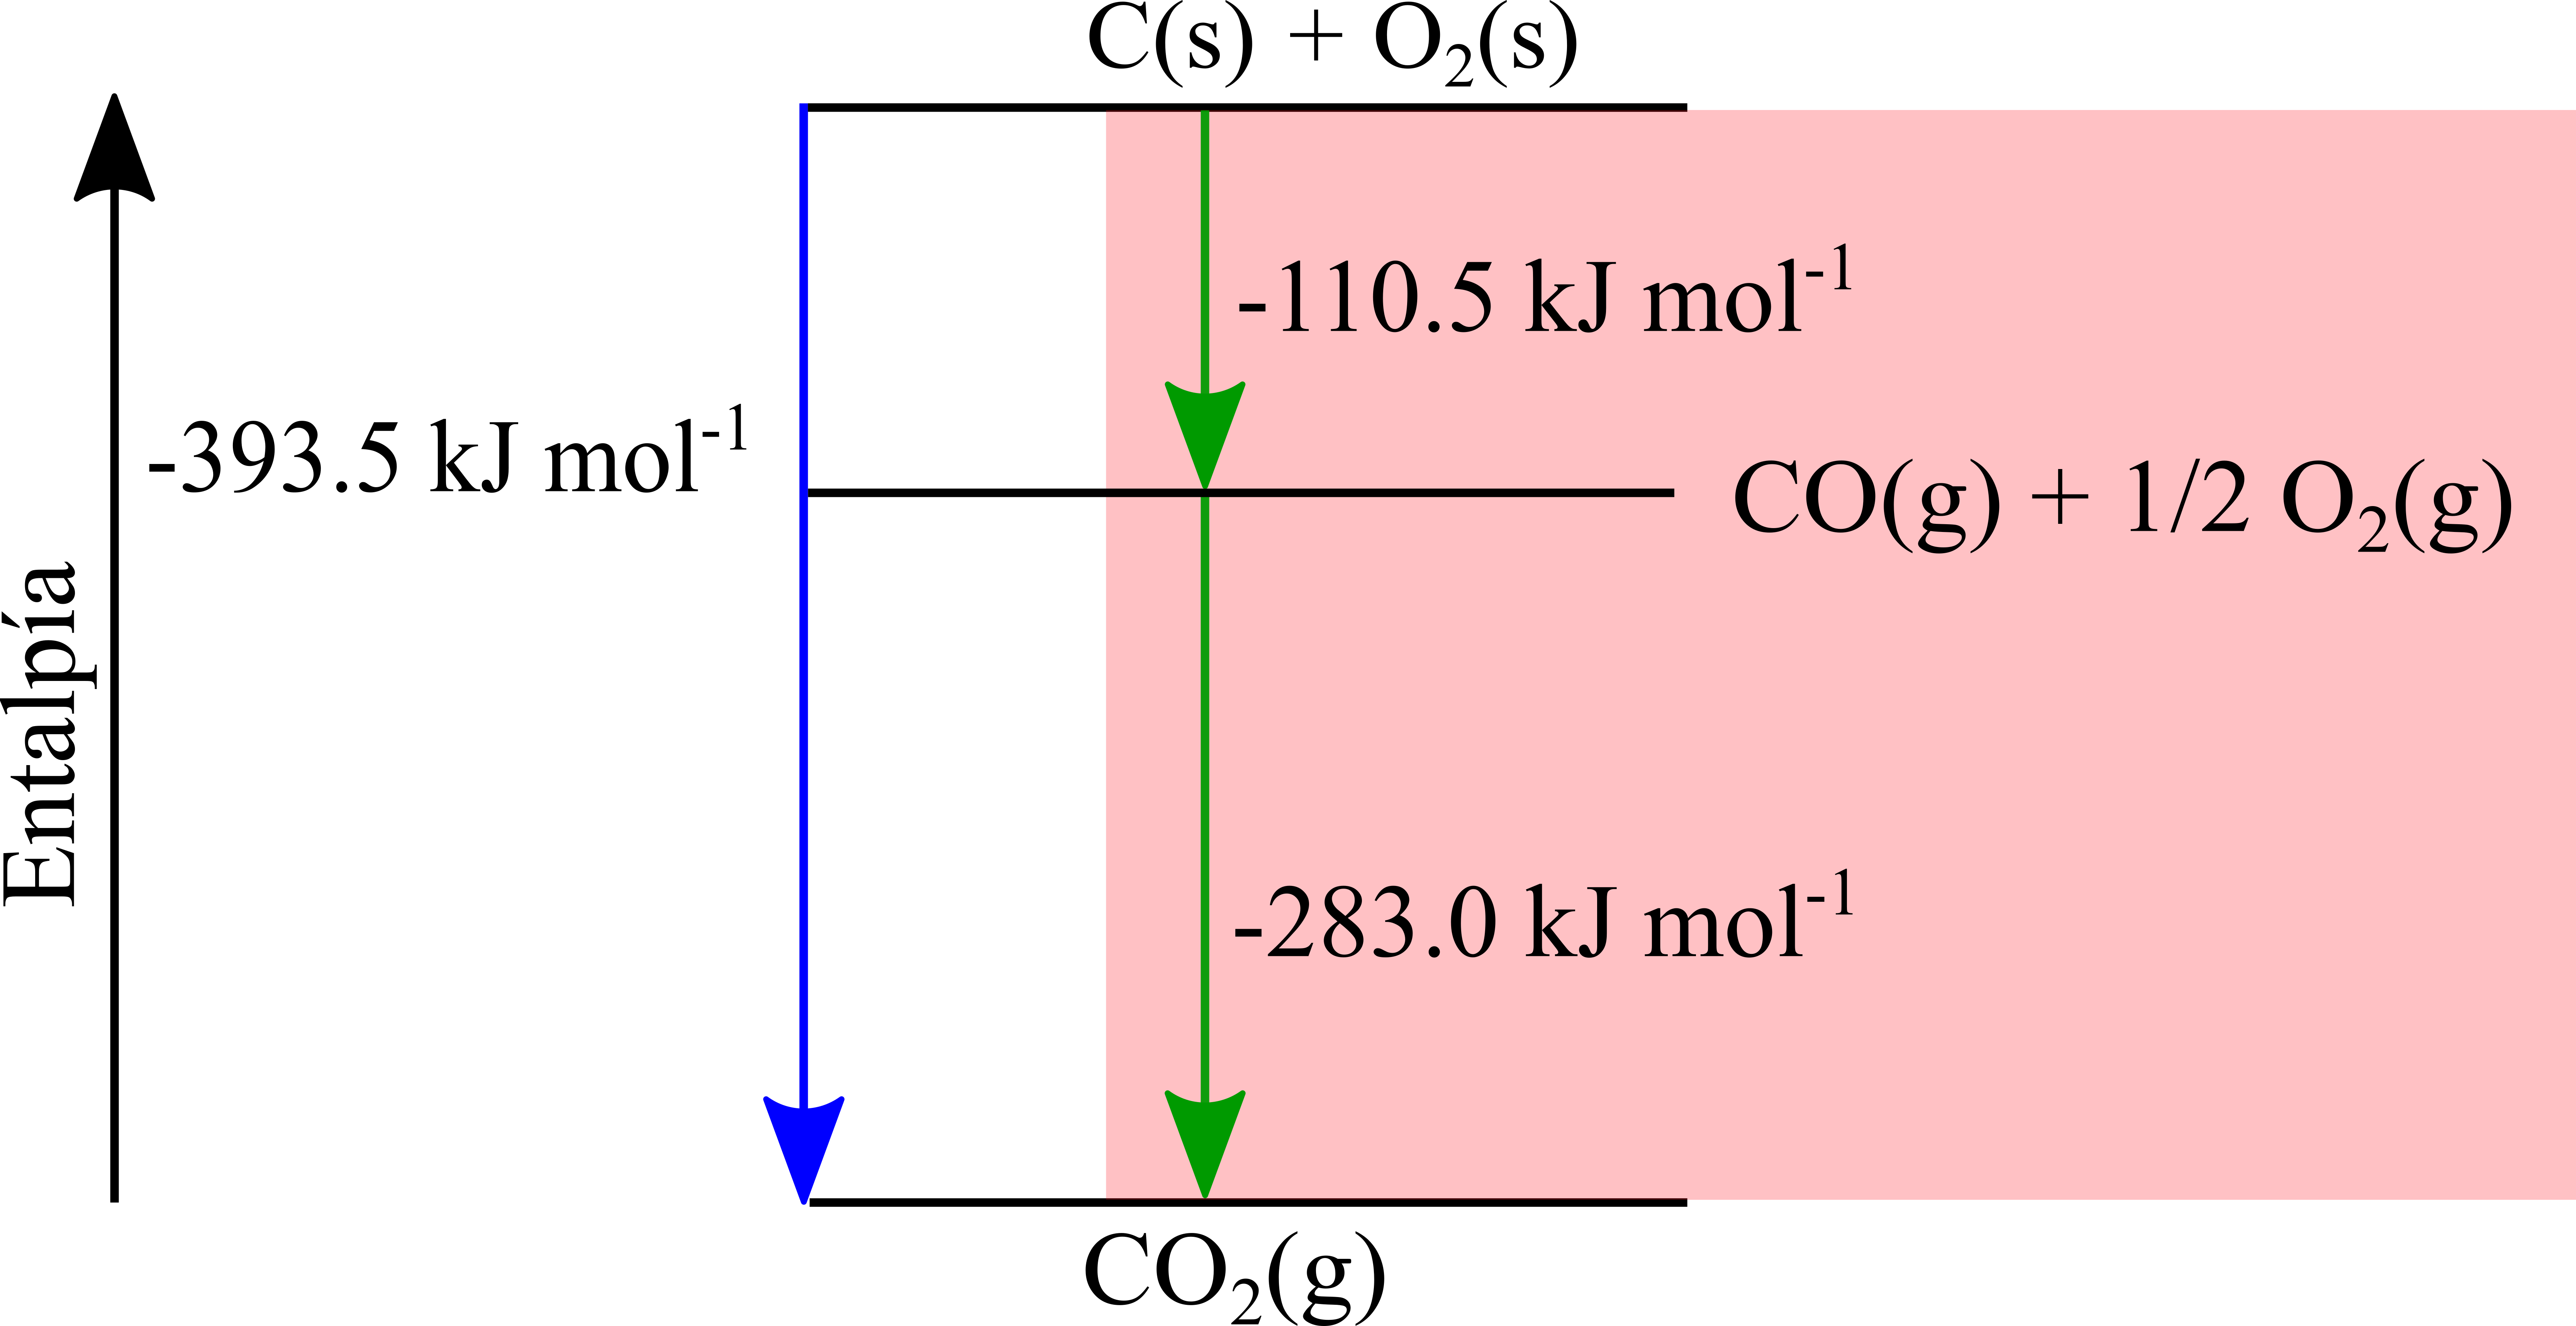
\includegraphics[scale=0.6]{graphs/CO.png}
\caption[Figura de la entalpía de formación de monóxido de carbono.]{Entalpía de formación de monóxido de carbono. El cambio de entalpía de la reacción total es igual a la suma de los cambios de entalpía de los dos pasos.}
\label{CO}
\end{center}
\end{figure}

\section{Química computacional}
Los métodos comentados en la sección \ref{sec:Hess}, permiten calcular los cambios de entalpía para una gran cantidad de reacciones (hay extensas tablas de entalpías de vaporización, entalpías de fusión y entalpías de combustión) \cite{NIST1998, Tajti2004, Nicolaides1996}. No obstante, también es posible cuantificar la entalpía de formación mediante cálculos \textit{ab initio} \cite{Lewars2016}.\\

La determinación de entalpías de formación por métodos computacionales es fundamental, porque sirve como información de entrada para multitud de simulaciones numéricas. Tal es la importancia, que se ha invertido un gran esfuerzo en la tabulación y refinamiento de \textit{JANAF}\cite{NIST1998}, \textit{CODATA}\cite{Cox1989}, \textit{Third Millenium}\cite{Goos1998} y \textit{Active Thermochemical Tables (ATcT)}\cite{Ruscic2004, Ruscic2005, Ruscic2005b}. Aunque la determinación experimental (principalmente mediante calorimetría) es el método más usado para obtener $\enthalpy*(f){}$, es a la vez, laborioso y consume mucho tiempo. Es claro que obtener $\enthalpy*(f){}$ experimental para todos los compuestos existentes es imposible y costoso. No obstante, ahora se acepta que la química teórica, ya sea de forma aislada o en conjunto con el experimento, pueda ofrecer un medio eficaz para obtener esta información.\\

La búsqueda del ``cielo químico'' en química computacional esta sujeto en gran medida, al tipo de metodología que sea capaz de predecir entalpías de formación con desviaciones menores a 4.184 kJ mol$^{-1}$ respecto al valor experimental. Por lo tanto, la precisión de cualquier $\enthalpy*(f){}$ depende del modelo químico aplicado y del tamaño del sistema molecular. Los métodos compuestos ofrecen una alternativa rentable a expensas de la precisión y consisten en una serie de optimizaciones de la geometría y cálculos de energía en un solo punto, con correcciones empíricas para superar las deficiencias cuando los métodos son comparados con entalpías de formación conocidas. Numerosos métodos se han usado en los últimos tiempos; los métodos CBS-x \cite{Montgomery2000, Ochterski1996} (x = QBB3 y APNO) y Gaussian-x \cite{Pople1989,Curtiss1990, Curtiss1991, Curtiss1998, Curtiss2007} (x = 1, 2, 3, 4), que son empleados en cálculos cinéticos y termodinámicos, siendo de gran relevancia para la termoquímica. 

Variantes del método G3, tales como G3B3 \cite{Baboul1999} y G3MP2 \cite{Curtiss1999} también son populares. El método G3 se emplea con frecuencia para la $\enthalpy*(f){}$ reportada por Burcat \textit{et al.} como parte de la base de datos \textit{Third Millenium}, con una incertidumbre de 8 kJ mol$^{-1}$. Los métodos ``estándar'' se han ajustado en numerosas ocasiones para remediar las dificultades percibidas con el objetivo de mejorar el coste computacional; un ejemplo de ello, son las variantes  de G4 \cite{Chan2010, Chan2011}, W1 \cite{Chan2012, Karton2012} y W3 \cite{Chan2013, Gruzman2009}. Para superar las grandes incertidumbres y errores en $\enthalpy*(f){}$ se emplea el método isodésmico, sin embargo, surge  un gran número de problemas al emplear este método porque se requieren entalpías de formación experimentales o métodos computacionales con un alto nivel de teoría para crear estas reacciones de trabajo hipotéticas;  los $\enthalpy*(f){}$ calculados dependen de la calidad de la reacción isodésmica (dado que no hay una única respuesta), además, el costo computacional se incrementa bastante. Pese a esto, los métodos computacionales pueden ofrecer excelentes resultados \cite{Simmie2015}.

\section{Métodos Gaussianos}

La clave de estos métodos es el uso de altos niveles de correlación y grandes conjuntos de bases. Esta serie comenzó en 1989 con \textit{Gaussian 1}, G1 \cite{Pople1989}, continuó con G2 (1991) \cite{Curtiss1991}, G3 (1998) \cite{Curtiss1998}, y G4 vio la publicación en 2007 \cite{Curtiss2007}. G1 y G2 están obsoletos. Los métodos Gaussianos de alta precisión más populares en la actualidad son probablemente G4 y G3 en conjunto de sus variantes más rápidas, G4(MP2) \cite{Curtiss2007a} y G3(MP2) \cite{Curtiss1999}. El uso continuo de G3 y G3(MP2) con G4 y G4(MP2) puede estar justificado por el deseo de comparar algunos trabajos actuales con resultados de métodos más antiguos. Para G3, la desviación absoluta media del experimento es de 4.7 kJ mol$^{-1}$, para G3(MP2)  es de 5.0 – 5.4 kJ mol$^{-1}$, es importante resaltar que G3(MP2) es de 7 a 8 veces más rápido que G3 \cite{Curtiss1998}. Para acelerar el método G4, sus pasos MP4 fueron reemplazados por MP2 y MP3 dando como resultado G4(MP2) y G4(MP3) \cite{Curtiss2007a, Lewars2016}. \\ Un cálculo G4, utiliza los siguientes pasos:
 
\begin{enumerate}
\item Obtención de la estructura de equilibrio en un nivel B3LYP/6-31G(2\textit{df,p}).
\item Especificación de las frecuencias armónicas.
\item Determinación de límite de energía Hartree-Fock.
\item Corrección de la energía.
\item Evaluación de la energía MP4/6-31G(\textit{d}), correcciones del paso anterior y combinación aditiva con el paso 3. 
\item Especificación de un nivel alto (HLC) con parámetros empíricos.
\item Obtención de la energía total a \textit{T} = 0 con una corrección en la energía de punto zero obtenida en el paso 2. 
\end{enumerate}

Estos siete pasos se utilizan para calcular una energía molecular como la suma de varias diferencias de energía y un incremento de energía empírica final (la ``corrección de nivel superior’’) en función del número de electrones apareados y no apareados. Debido a las correcciones de energía empírica en los métodos  gaussianos, no son completamente \textit{ab initio}, sino algo \textit{semiempíricos}, excepto cuando estas correcciones se anulan. Esta cancelación ocurre, por ejemplo, al calcular las afinidades de los protones como la diferencia de energía de las especies protonadas y no protonadas. Los métodos gaussianos, CBS y otros no mencionados aquí, son revisados  por Peterson, Feller y Dixon en el año 2012, con énfasis en termoquímica; estos autores reconocen una precisión química de 4 kJ mol$^{-1}$ como aceptable \cite{Peterson2012}. \\

\section{Métodos CBS}
En estos métodos se usa una extrapolación del conjunto de bases a un límite infinito (hasta el final). Hay tres métodos CBS básicos: CBS-4 (para extrapolación de cuarto orden), CBS-Q (para CI cuadrático) y CBS-APNO (para orbitales naturales de pares asintóticos, referidos a la extrapolación al límite establecido de base). Dichos métodos están disponibles en los programas \textit{Gaussian 94} y posteriores. CBS-4M puede manejar moléculas con hasta 19 átomos pesados. Los errores CBS-4M más típicos son (desviación absoluta media del experimento) 13.6 kJ mol$^{-1}$ \cite{Montgomery2000}. Hay una modificación de CBS-4M diseñada para disminuir la acumulación de errores con el aumento del tamaño molecular. CBS-QB3 puede manejar moléculas con hasta 13 átomos pesados y tiene una desviación media absoluta del experimento de 4.6 kJ mol$^{-1}$ \cite{Montgomery1999}. CBS-APNO puede manejar moléculas con hasta 7 átomos pesados y tiene una desviación absoluta media del experimento de 2.2 kJ mol$^{-1}$ \cite{Irikura1998}. Este conjunto de métodos implican esencialmente siete u ocho pasos \cite{Lewars2016}:

\begin{enumerate}
\item Una optimización de geometría (en el nivel HF/3–21G(*) o MP2/6–31G*, dependiendo del método CBS en particular).

\item Cálculo de ZPE a nivel de optimización.

\item Determinación de punto único de HF con un conjunto de bases muy grande (6–311 + G(3d2f,2df,p) o 6–311 + G(3d2f,2df,2p), dependiendo del método CBS).

\item Cálculo de punto único MP2 (base que depende del método CBS).

\item Extrapolación de un par de orbitales naturales para estimar el error debido al uso de un conjunto de bases finitas.

\item Determinación de energía MP4.

\item Para algunos métodos CBS, un cálculo de punto único QCISD(T).

\item Una o más correcciones empíricas, teniendo en cuenta el aspecto semiempírico de los métodos CBS. 

\end{enumerate}


\section{Comparacion entre métodos} 
En este trabajo nos concentraremos en los métodos de tipo gaussiano y CBS (en especial de tipo gaussiano), porque estos han sido los más utilizados, y por lo tanto, han acumulado una gran cantidad de resultados publicados, además de ser los más accesibles. Sin embargo, como ya mencionamos, existen otros métodos de alta precisión, como los procedimientos de Weizmann de Martin y de Oliveira, W1 y W2 \cite{Martin1999},  Boese \textit{et al.} W3 y W4 \cite{Boese2004} y las modificaciones más rápidas de estos como W2X y W3X-L de Chan y Radom \cite{Chan2015}, los cuales, al igual que los métodos CBS, se basan en la extrapolación de conjuntos de bases. El autor principal de esta revisión es el profesor K. A. Peterson de la Universidad Estatal de Washington; los métodos CBS provienen del grupo de investigación del profesor G. A. Petersson de la Universidad Wesleyana; ambos investigadores están activos en termoquímica cuántica computacional.\\

De los métodos de tipo gaussiano y CBS, para una alta precisión en moléculas muy pequeñas, CBS-APNO es la elección adecuada, y para moléculas "grandes", la elección recae en CBS-4M con la aceptación de la posibilidad de errores moderadamente grandes. Para moléculas de tamaño intermedio, la mejor elección es probablemente entre G4(MP2) y CBS-QB3. Recordemos que G4(MP2) es mucho más rápido que G4, con poca pérdida de precisión en la mayoría de los casos \cite{Lewars2016}.\\

\begin{comment}
En la tabla \ref{Fattahi-table} se muestra una comparación de los métodos gaussianos y un método CBS, usando 1,4-benzoquinona (p-benzoquinona, $O=C_{6}H_{4}=O$) al calcular la entalpía de formación por el método de atomización. Se debe tener en cuenta que el cálculo G4 tomó nueve veces más tiempo (160/18) que el G4 (MP2) y ambos dieron casi la misma entalpía de formación \cite{Lewars2016}. 

\begin{table}[H]
\begin{center}
\begin{tabular}{||l|c|c||}
\hline 
Método & $\Delta_{f}$H/(kJ mol$^{-1})$ & minutos/tiempo relativo \\ 
\hline 
G4 & -117.5 & 160/21 \\ 
\hline 
G4(MP2) & -118.5 & 18/2.4 \\ 
\hline 
G3 & -118.6 & 24/3.2 \\ 
\hline 
G3(MP2) & -120.0 & 7.5/1 \\ 
\hline 
CBS-QB3 & -115.9 & 16/2.1 \\ 
\hline 
\end{tabular} 
\end{center}
\caption[La entalpía de formación aceptada en la literatura es de -122. $\pm$ 3.8 kJ mol$^{-1}$ \cite{Fattahi2005}.]{Los primeros cuatro valores calculados experimentalmente están dentro de 1 kJ mol$^{-1}$, sin embargo, el valor CBS-QB3 es de 3 kJ mol$^{-1}$ y está por encima del mayor error estimado. No obstante, no se debe generalizar a partir de una muestra de un solo compuesto.}
\label{Fattahi-table}
\end{table}

\end{comment}

\section{Método de atomización} 

En química computacional hay tres enfoques principales que predicen entalpías de formación. 

\begin{enumerate}
\item Método de atomización.
\item Método de formación.
\item Método de reacciones isodésmicas.
\end{enumerate}

 
De los 3 enfoques anteriores, el método de atomización da mejores resultados, especialmente para moléculas orgánicas y es el más sencillo, porque se basa en la ruptura de enlaces de una molécula para obtener a sus átomos en fase gas\cite{Nicolaides1996}. A continuación se analizará el principio del método de atomización con la molécula de metanol. \\

La entalpía de atomización, $\Delta_{\mathrm{a}} H^{\circleddash}_{T}$ a \textit{T} = 0 \textit{ab initio}, del metanol es la diferencia de entalpía entre los átomos de la molécula y el metanol. Para calcular $\Delta_{\mathrm{f}}H^{\circleddash}_{0}$ se requiere la entalpía de formación a \textit{T} = 0 de los átomos de C, H y O y la entalpía de atomización a \textit{T} = 0 del metanol (ecuaciones \ref{eq:3.14} y \ref{eq:3.15}). Las entalpías de atomización del hidrógeno y el oxígeno se pueden calcular por un método \textit{ab initio}, pero no de forma fiable y precisa. Para mantener la coherencia, utilizaremos valores experimentales de las tres entalpías de atomización elementales, como recomiendan Nicolaides \textit{et al.}\cite{Nicolaides1996}. De la ecuación \ref{eq:3.16}, la entalpía de atomización \textit{T} = 0 del metanol es simplemente las suma de las entalpías \textit{ab initio} de los átomos que la constituyen menos la entalpía \textit{ab initio} corregida por ZPE del metanol:

\begin{equation}
	\Delta_{\mathrm{f}} H^{\circleddash}_{0}(\mathrm{CH_3OH}) + \Delta_{\mathrm{a}} H^{\circleddash}_{0} (\mathrm{CH_{3}OH}) = \Delta_{\mathrm{f}} H^{\circleddash}_{0} \mathrm{(C(^{3}P) + 4H(^{2}S) + O(^{3}S))}
\label{eq:3.14}
\end{equation}\\

\begin{equation}
	\Delta_{\mathrm{f}} H^{\circleddash}_{0}(\mathrm{CH_3OH}) = \Delta_{\mathrm{f}} H^{\circleddash}_{0} \mathrm{(C(^{3}P) + 4H(^{2}S) + O(^{3}S))} - \Delta_{\mathrm{f}} H^{\circleddash}_{0} \mathrm{(CH_3OH)}
\label{eq:3.15}
\end{equation}\\

\begin{equation}
	\Delta_{\mathrm{a}} H^{\circleddash}_{0}(\mathrm{CH_3OH)} = \Delta E^{total}_{0\mathrm{K}} \mathrm{(C(^{3}P) + 4H(^{2}S) + O(^{3}S))} - \Delta E^{total}_{0\mathrm{K}}(\mathrm{CH_3OH)}
\label{eq:3.16}
\end{equation}\\

\begin{figure}[H]
\begin{center}
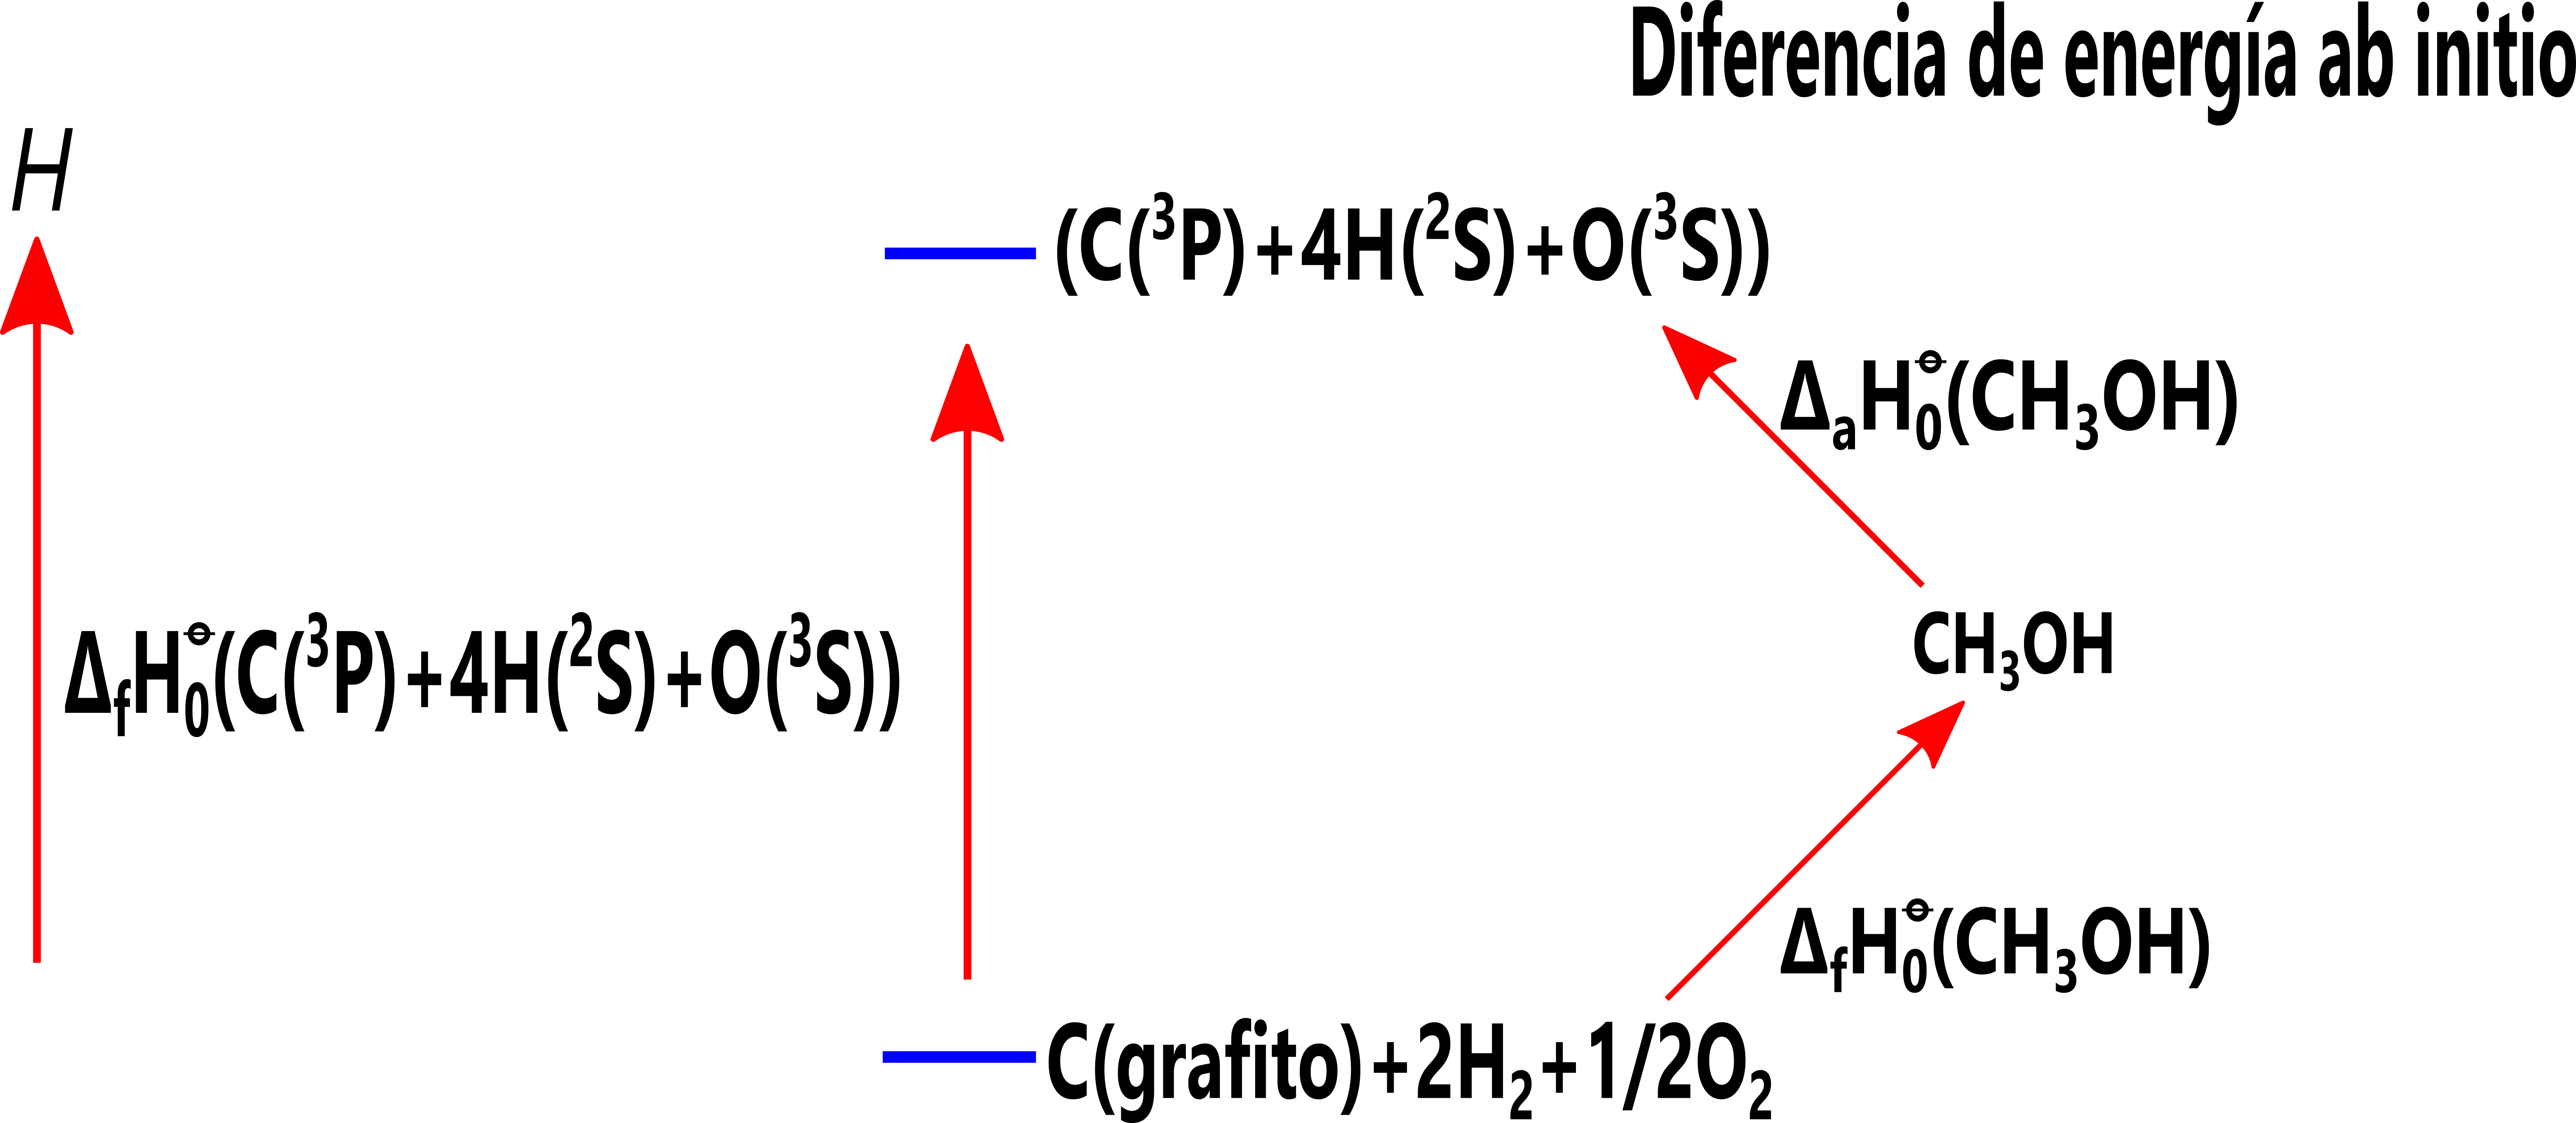
\includegraphics[scale=.6]{graphs/atomization-CH3OH.png}
	\caption[Figura de entalpía de atomización de metanol.]{El metanol se atomiza (conceptualmente) a \textit{T} = 0 en los átomos que lo constituyen, es decir,  carbono, hidrógeno y oxígeno (en sus estados electrónicos fundamentales). Además, los átomos de la molécula en sus estados estándar también son usados para formar dicha molécula. La entalpía de formación del metanol a \textit{T} = 0, $\Delta_{\mathrm{f}} H^{\circleddash}_{0}$(CH$_3$OH), se obtiene al igualar la energía necesaria para generar los átomos a través del metanol ($ \Delta_{\mathrm{f}} H^{\circleddash}_{0}$(CH$_3$OH) + $ \Delta_\mathrm{{a}} H^{\circleddash}_{0}$(CH$_3$OH)) a la energía para hacerlo directamente desde sus elementos en sus estados estándar \cite{Lewars2016}.}
\label{atm-metanol}
\end{center}
\end{figure}

Los valores experimentales de las entalpías de atomización de los átomos a \textit{T} = 0 de $\mathrm{(C(^{3}P) + 4H(^{2}S) + O(^{3}S))}$ se ilustran en la tabla \ref{Nicolaides-table}.

\begin{table}[H]
\begin{center}
\begin{tabular}{||c|c||}
\hline 
Átomo  & Entalpía experimental/(kJ mol$^{-1}$) \\ 
\hline 
\hline
C & 711.185 \\ 
\hline 
H & 216.03500 \\ 
\hline 
O & 246.7900 \\ 
\hline 
\end{tabular}
	\caption{Entalpías de formación experimentales reportadas por Nicolaides \textit{et al.} \cite{Nicolaides1996}.}
\label{Nicolaides-table}
\end{center}
\end{table}

Posteriormente, para calcular $\Delta_{\mathrm{a}} H^{\circleddash}_{0} \mathrm{(CH_3OH)}$ se usará la ecuación \ref{eq:3.16} que toma el valor de $\Delta E^{total}_{0\mathrm{K}}$ para los átomos de  C, H, y O. En lugar del método G2 que fue empleado por Nicolaides \textit{et al.} \cite{Nicolaides1996}, usaremos el método G4 de \textit{Gaussian09}. Los valores obtenidos para cada átomo y su respectiva molécula a \textit{T} = 0 se muestran en la tabla \ref{G4-table}.\\


\begin{table}[H]
\begin{center}
\begin{tabular}{||c|c||}
\hline 
	Átomos  & Entalpías G4 a \textit{T} = 0  (hartrees) \\ 
\hline
\hline 
C & -37.834170 \\ 
\hline 
H & -0.501420 \\ 
\hline 
O & -75.045500 \\ 
\hline 
CH$_{3}$OH & -115.651767 \\
\hline
\end{tabular}
	\caption{Entalpías de formación a \textit{T} = 0 obtenidas por el método G4 de Gaussian09.}
\label{G4-table}
\end{center}
\end{table}


El valor de metanol de $-115.651767$ h podría llamarse el ``cero absoluto'' de la entalpía del metanol, es decir, la entalpía relativa a la de los núcleos disociados y electrones. Esta entalpía absoluta se utilizará en el cálculo de la entalpía de formación. De la ecuación \ref{eq:3.16} es posible calcular la energía de atomización de metanol a \textit{T} = 0:

\begin{multline}
	\Delta_{\mathrm{a}} H^{\circleddash}_{0}\;\mathrm{(CH_3OH)} = -37.834170\;\mathrm{h} + 4(-0.501420)\;\mathrm{h}-75.045500\;\mathrm{h}-(-115.651767)\;\mathrm{h} =...\\
	...= (0.766417\;\mathrm{h})(2625.5\;\mathrm{kJ\;mol^{-1}}) = 2012.227\;\mathrm{kJ\;mol^{-1}}
\label{eq:3.17}
\end{multline}\\

De la ecuación \ref{eq:3.14} la entalpía de formación a \textit{T} = 0 de metanol es:\\

\begin{multline}
	\Delta_{\mathrm{f}} H^{\circleddash}_{0}\mathrm{(CH_3OH)} = 711.185\;\mathrm{kJ\;mol^{-1}} + 4(216.03500)\;\mathrm{kJ\;mol^{-1}} +... \\...\; 246.7900\;\mathrm{kJ\;mol^{-1}}- 2012.227\;\mathrm{kJ\;mol^{-1} = -190.112\;kJ\;mol^{-1}}
\label{eq:3.18}
\end{multline}\\

Nicolaides \textit{et al.} \cite{Nicolaides1996} reportaron un valor de 195.7 kJ mol$^{-1}$ a \textit{T} = 0 mediante el método de atomización junto con los valores experimentales, que son 190.7 kJ mol$^{-1}$ y 189.8 kJ mol$^{-1}$, que concuerdan con el valor G4 calculado aquí. Cualquier inexactitud en la energía de atomización calculada, se mostrará en la entalpía de formación, y solo un buen método de alta precisión puede mitigar este error de manera confiable. Para ajustar la entalpía de formación de \textit{T} = 0 a \textit{T} = 298 K, debemos agregar dicho valor y restar los aumentos correspondientes para los elementos en sus estados estándar. El valor para el metanol es la diferencia de las dos cantidades G4 proporcionadas en el archivo de salida de Gaussian. El aumento de la entalpía del metanol al pasar de \textit{T} = 0 a \textit{T} = 298 K es:


\begin{equation}
	\Delta \Delta H^{\circleddash}(\mathrm{CH_3OH}) = \mathrm{G4}\;\textrm{Entalpía} - \mathrm{G4} \;(0\mathrm{K})
\label{eq:3.19}
\end{equation}\\

\begin{multline}
	\Delta \Delta H^{\circleddash}\mathrm{(CH_3OH)} = -115.647489\;\mathrm{h} - (-115.651767\;\mathrm{h})\; =...\\
	...= (0.004278\;\mathrm{h})(2625.5\;\mathrm{kJ\;mol^{-1})} = 11.23188\;\mathrm{kJ\;mol^{-1}}
\label{eq:3.20}
\end{multline}\\

Las entalpías experimentales de los respectivos elementos también es reportada por Nicolaides \textit{et al.}\cite{Nicolaides1996} en kJ mol$^{-1}$, véase la tabla \ref{Nicolaides-exp-table}.

\begin{table}[H]
\begin{center}
\begin{tabular}{||c|c||}
\hline 
	Átomos  & Entalpía experimental/($\mathrm{kJ\;mol^{-1}}$) \\ 
\hline 
C(grafito) & 1.05100 \\ 
\hline 
H$_{2}$ & 8.46700 \\ 
\hline 
O$_{2}$ & 8.67000 \\ 
\hline 
\end{tabular}
	\caption{Entalpías experimentales de los elementos reportadas por Nicolaides \textit{et al.}\cite{Nicolaides1996}.}
\label{Nicolaides-exp-table}
\end{center}
\end{table}

Ahora, para ajustar la entalpía de formación a un estado estándar, sumamos el aumento de entalpía del metanol al pasar de \textit{T} = 0 a \textit{T} = 298 K y restamos los aumentos correspondientes de los elementos en sus estados estándar.

\begin{multline}
	\enthalpy*(f){} \mathrm{(CH_3OH)} = \Delta_{\mathrm{f}} H_{0}^{\circleddash}\mathrm{(CH_{3}OH)} + \Delta \Delta H^{\circleddash} \mathrm{(CH_{3}OH)} \\ - (\Delta \Delta H^{\circleddash} \mathrm{(C)} + 2 \Delta \Delta H^{\circleddash}(\mathrm{H_{2}}) + \frac{1}{2} \Delta \Delta \mathrm{H}^{\circleddash}\mathrm{(O_{2}))}
\label{eq:3.21}
\end{multline}\\

\begin{multline}
	\enthalpy*(f){} \mathrm{(CH_3OH)} = -190.112\;\mathrm{kJ\;mol^{-1}} + 11.23188\;\mathrm{kJ\;mol^{-1}}  \\ - (1.05100 + 2(8.467000) + \frac{1}{2} (8.6700))\;\mathrm{kJ\;mol^{-1}}
\label{eq:3.22}
\end{multline}\\

\begin{equation}
	\enthalpy*(f){} \mathrm{(CH_3OH)} = -201.20\;\mathrm{kJ\;mol^{-1}}
\label{eq:3.23}
\end{equation}\\

El valor experimental a \textit{T} = 298 K aceptado es de -205 $\pm$ 10 kJ mol$^{-1}$\cite{Afeefy2009}. Por lo tanto, la cifra calculada está dentro del error experimental esperado \cite{Lewars2016}.


\section{Relaciones Generales de Termodinámica Estadística}

Algunos métodos computacionales, particularmente las técnicas \textit{ab initio}, producen información molecular detallada pero no información termodinámica directamente. Se necesitan más cálculos para generar cantidades como la entropía molar estándar (S°), la capacidad calorífica (C$_{p}$) y el cambio de entalpía \textit{[H°(T)-H°(0)]}. En algunos cálculos \textit{ab initio}, los resultados ni siquiera corresponden a las propiedades a temperatura de cero absoluto y siempre deben corregirse. Estas correcciones se basan en la Termodinámica Estadística, en dependencia de la función de partición molecular, $Q$. La función de partición se usa no solo para predicciones teóricas, sino también para generar la mayoría de las tablas termoquímicas publicadas. 

Los modelos \textit{ab initio} también  utilizan la aproximación Born-Oppenheimer. La base física de la aproximación de Born-Oppenheimer es que los núcleos son mucho más masivos que los electrones, por lo tanto, se mueven lentamente en relación con los electrones. En consecuencia, se puede considerar que los electrones se mueven en un campo producido por los núcleos fijados en alguna separación internuclear. Las energías resultantes son correctas para una molécula hipotética que no vibra. Aunque los osciladores pueden estar en reposo en la mecánica clásica, los osciladores reales (mecánica cuántica) siempre están en movimiento. El pequeño movimiento residual a la temperatura de cero absoluto es la energía vibracional de punto cero, abreviada como ZPVE o ZPE. Para un oscilador armónico simple, el ZPE es igual a la mitad de la frecuencia vibracional. Aunque todas las vibraciones moleculares reales son al menos ligeramente anarmónicas, por lo general se aproximan como armónicas. Así pues, la ZPE de una molécula puede calcularse como la mitad de la suma de las frecuencias vibracionales. En la ecuación \ref{eq:3.24}, $N$ es el número de átomos en la molécula, $\nu _{i}$ son las frecuencias vibracionales fundamentales. Hay vibraciones $3N-6$ en una molécula no lineal y $3N-5$ en una molécula lineal; la ecuación \ref{eq:3.24} es para el caso no lineal. El ZPE debe agregarse a la energía \textit{ab initio} para obtener una energía correspondiente a \textit{T} = 0.

\begin{equation}
ZPE = \frac{1}{2} \sum_{i=1}^{3N-6} \nu_{i}
\label{eq:3.24}
\end{equation}\\

En la práctica, la corrección ZPE se complica un poco debido a que las
frecuencias vibracionales \textit{ab initio} a menudo tienen un error de $+5\%$ a $+10\%$. Para compensar este error, las frecuencias calculadas generalmente se multiplican por factores de escala empíricos. Las recomendaciones más recientes son las de Scott \textit{et al.} \cite{Scott1996}. Por ejemplo, sugieren escalar las frecuencias HF/6-31G* en 0.8953 para predecir espectros de vibración (es decir, frecuencias fundamentales), en 0.9135 para el cálculo de ZPE, en 0.8905 para predecir diferencias de entalpía $[H^{\circ}(298.15) - H^{\circ}(0)]$.\\

La Termodinámica Estadística pretende incluir los métodos utilizados para convertir los niveles de energía molecular en propiedades macroscópicas, especialmente entalpías, entropías y capacidades caloríficas. Los niveles de energía molecular surgen de la traslación molecular (es decir, el movimiento a través del espacio), la rotación, la vibración y la excitación electrónica. Esta información constituye la espectroscopia de la molécula de interés y puede obtenerse experimentalmente o mediante cálculos \textit{ab initio} \cite{Irikura1998}. \\

\subsection{Función de partición}

Los niveles de energía molecular $\varepsilon_{i}$ se utilizan para calcular la función de partición molecular, generalmente denotada por el símbolo $Q$, como se muestra en la ecuación \ref{eq:3.25} (se extiende sobre todos los niveles de energía). 

\begin{equation}
Q(T) =  \sum_{i=1} e^{-\frac{\varepsilon_{i}}{kT}}
\label{eq:3.25}
\end{equation}\\

Sin embargo, para temperaturas muy altas donde las moléculas se vuelven inestables, la extensión de la suma puede ser ambigua. Los datos termoquímicos tabulados deben utilizarse con precaución en tales condiciones porque los valores (1) pueden depender en gran medida del procedimiento de energía adoptado y (2) pueden desviarse implícitamente del modelo de gas ideal. Normalmente, uno elige el nivel de energía más bajo para que sea el cero de energía, de modo que ningún nivel se encuentre en energías negativas. De la ecuación \ref{eq:3.25} se deduce que las mayores contribuciones para $Q$ provienen de los niveles de energía más bajos. Por el contrario, los niveles que se encuentran muy por encima de \textit{kT} (207 cm$^{-1}$ a temperatura ambiente) tienen solo un efecto menor sobre $Q$ y sus cantidades termodinámicas derivadas \cite{Irikura1998}.\\

\subsection{Funciones termodinámicas}

Dada la función de partición, se pueden calcular las funciones termodinámicas habituales. No obstante, aquí solo usaremos las ecuaciones que permiten calcular la diferencia relativa de entalpía, véase la ecuación de Kirchhoff (ecuación \ref{eq:3.26}) \cite{Irikura1998}.

\begin{equation}
H(T)-H(0) = \int_{0} ^{T} C_{p} dT = \frac{RT^{2}}{Q} \frac{\partial Q}{\partial T} + RT
\label{eq:3.26}
\end{equation}

\subsection{Cálculos prácticos}

Casi nunca se dispone de un conjunto completo de niveles de energía molecular. Para
simplificar el problema, se suele adoptar un modelo en el que la traslación, la rotación, la vibración y la excitación electrónica están desacopladas. En otras palabras, se asume que la aproximación de los diferentes tipos de movimiento no se afectan entre sí y no se mezclan. Esto conduce  a separar $Q$ en cuatro factores que corresponden a funciones de partición separadas para traslación, rotación, vibración y excitación electrónica. Esto se muestra en la ecuación \ref{eq:3.27}.

\begin{equation}
Q = Q_{tras}Q_{rot}Q_{vib}Q_{elec}
\label{eq:3.27}
\end{equation}\\

Cuando se consideran los estados electrónicamente excitados, a menudo se supone que
los espectros de traslación, rotación y vibración del estado excitado son los mismos que los del estado electrónico fundamental. Esto es conveniente cuando no hay otra información disponible. Además, si el estado excitado se encuentra muy por encima de \textit{kT}, los resultados finales no serán sensibles a tales detalles \cite{Irikura1998}. \\


\subsection{Función de partición traslacional}

$Q_{tras}$ debe calcularse a partir de una suma de todos los niveles de
energía de traslación que están disponibles para una molécula confinada en una caja
cúbica de volumen \textit{V = RT/p} (volumen molar de un gas ideal a temperatura \textit{T} y presión $p$).Esto rara vez se hace. En cambio, la suma se aproxima como una integral para obtener la ecuación \ref{eq:3.28}. Esta aproximación es buena siempre que $m^{3/2}/T^{5/2}$ $p^{-1}$ $\gg$ $h^{3}(2\pi)^{-3/2}k^{-5/2}$. Cuando $p$ = 1 bar, esta condición se cumple para moléculas suficientemente pesadas, $m$ (en uma) $\gg$ $11.4 T^{-5/3}$ y para temperaturas suficientemente altas, \textit{T} $\gg$ $4.31 m^{-3/5}$. Afortunadamente, esto cubre las condiciones de interés químico. Para un gas ideal monoatómico, no hay movimiento vibratorio o rotacional \cite{Irikura1998}.\\

\begin{equation}
[H(T)-H(0)]_{tras} = \frac{3}{2} RT
\label{eq:3.28}
\end{equation}\\

\newpage

\subsection{Función de partición rotacional}

La rotación libre de una molécula rígida también está cuantizada (el momento angular y su proyección son múltiplos enteros de $h/2\pi$), por lo que la energía de rotación está restringida a ciertos niveles discretos. Los espectros de rotación se caracterizan por las constantes $A, B, C$, donde $A \equiv$ $h/(8\pi^{2}I_{A}$) y lo mismo para $B$ y $C$. Las cantidades $I_{A,B,C}$ son los momentos principales de inercia de la molécula, con la convención $I_{A} \leq I_{B} \leq I_{C}$ (o $A \geq B \geq C$). Muchos programas, incluidos los paquetes \textit{ab initio}, informan las constantes de rotación cuando se les proporciona una geometría molecular. Los momentos también se pueden calcular manualmente como los valores propios del tensor de inercia, que tiene elementos como $I_{xy} = - \sum m_{i}x_{i}y_{i}$ y $I_{xx} = + \sum m_{i}x_{i}(y_{i}^{2}+z_{i}^{2})$, donde el índice $i$ recorre todos los átomos en la molécula y el origen de coordenadas está en el centro de masa. Las moléculas lineales $(I_{A} = 0)$ se describen mediante una sola constante de rotación $B$, y no solo por el momento de inercia, $I$. Afortunadamente, a temperaturas lo suficientemente altas ($kT \gg hA$), la suma se puede reemplazar por una integral como lo es para la traslación. En el caso general, la función de partición rotacional viene dada por la ecuación \ref{eq:3.29}. Para moléculas lineales, se debe usar la ecuación \ref{eq:3.30} en su lugar \cite{Irikura1998}.


\begin{equation}
[H(T)-H(0)]_{rot} = \frac{3}{2} RT
\label{eq:3.29}
\end{equation}


\begin{equation}
[H(T)-H(0)]_{rot}^{lineal} =  RT
\label{eq:3.30}
\end{equation}

\newpage

\subsection{Función de partición vibracional}

Para completar el modelo simple de rotor rígido/oscilador armónico (RROA), se deben
considerar las vibraciones moleculares. Como se indica en la discusión de ZPE (ecuación
\ref{eq:3.24}), una molécula que contiene $N$ átomos tiene $3N-6$ frecuencias vibratorias o $3N-5$ para moléculas lineales. Las función de partición para la entalpía está dada por la ecuación \ref{eq:3.31} \cite{Irikura1998}.

\begin{equation}
[H(T)-H(0)]_{vib}=RT \sum_i \left(\frac{h\nu_i}{kT}\right)\left(\frac{e^{\frac{-h\nu_i}{kT}}}{1-e^{\frac{-h\nu_i}{kT}}}\right)
\label{eq:3.31}
\end{equation}

\subsection{Función de partición electrónica}

Aunque es posible que no tengan excitación electrónica a baja temperatura estados, algunas moléculas tienen estados fundamentales electrónicos degenerados. Los radicales libres son un ejemplo común. Pueden tener electrones desapareados en sus estados básicos electrónicos y un espín electrónico neto de $S = n_{desapareado}/2$, donde $n_{desapareado}$ es el número de electrones desapareados. La multiplicidad, o degeneración $g$, de tal estado es $g = (2S+1)$. El uso de números de degeneración equivale a un recuento explícito de todos los estados, incluidos los degenerados. Por lo tanto, $Q_{elec} = g$ es una constante y solo afecta la entropía \cite{Irikura1998}.\\


\subsection{Cálculo de entalpía mediante Termodinámica Estadística}

Para calcular la entalpía se usan las ecuaciones \ref{eq:3.28}, \ref{eq:3.29}, \ref{eq:3.31} y \ref{eq:3.31}. Esto es $[H(298.15)-H(0)] = [H(T)-H(0)]_{vib}+[H(T)-H(0)]_{rot}+[H(T)-H(0)]_{tras}$. La contribución electrónica es ignorada (es decir, la función de partición correspondiente se establece en la unidad). Por otra parte, es posible remplazar la diferencia de las dos cantidades Gn o CBS proporcionadas en el resumen termoquímico  implementado en \textit{Gaussian} por el valor de la entalpía (energía interna) a partir de su función de partición \cite{Irikura1998}.


\section{Aproximación de Nicolaides}

 
Nicolaides \textit{et al.} en 1996, publicaron un artículo en el que intentaron corregir los posibles errores cuando existen rotores internos en moléculas. Por ejemplo, para el caso de la molécula de tolueno, el metilo que esta unido al anillo aromático puede estar girando, en consecuencia, es una mala idea usar la aproximación de rotor rígido/oscilador armónico, donde tendríamos un rotor rígido (en un rotor rígido la distancias relativas entre todas las partículas siempre es constante). Cuando una molécula gira o rota, pensaríamos que su geometría y distancias entre sus átomos nunca va a cambiar (ese es un error que se observa en la molécula de tolueno, porque el metilo rota de forma independiente). Y cuando suponemos a la molécula como un rotor rígido, estamos suponiendo que el metilo no rota, porque si rotase, la distancia relativa de los hidrógenos del metilo a los hidrógenos del anillo aromático cambiaría. Por lo tanto, ya no se cumpliría la definición de rotor rígido. No obstante, pensar en rotores rígidos, simplifica el problema matemático cuando se intenta calcular la función de partición, pero puede darnos errores con moléculas que contienen rotores internos. Es así, que se propone tratar a las rotaciones internas como rotores libres cuando las frecuencias vibraciones de las moléculas son menores a 260 cm$^{-1}$ y en su lugar utilizar $\frac{1}{2}$ de \textit{RT} para la contribución vibracional por cada frecuencia que sea menor a 260 cm$^{-1}$ \cite{Nicolaides1996}. Cuando esto no se cumpla, será necesario utilizar la aproximación de rotor rigido/oscilador armónico. Además, se debe añadir un \textit{RT} adicional a la energía interna para convertir a la energía en entalpía (el llamado término \textit{pV}). La ecuación general para el cálculo de la entalpía (energía interna) tendrá la siguiente forma, obsérvese la ecuación \ref{eq:3.32}.

\begin{equation}
[H(298.15)-H(0)] = [H(T)-H(0)]_{vib}+[H(T)-H(0)]_{rot}+[H(T)-H(0)]_{tras} + pV
\label{eq:3.32}
\end{equation}

\newpage

\section{Hardware y software}

Actualmente, las computadoras pueden realizar cálculos y tomar decisiones lógicas con una rapidez difícil de imaginar 
(miles de millones de cálculos en un segundo), más de lo que un humano podría realizar en toda su vida. 
Las computadoras procesan datos, bajo el control de un conjunto de instrucciones conocidas como programas de computadora. 
Estos programas guían a la computadora a través de conjuntos ordenados de acciones especificadas por gente conocida como programadores. 
A los programas que se ejecutan en una computadora se les denomina \textit{software}. A las partes de una computadora que consisten en varios dispositivos se les conoce como \textit{hardware} (teclado, pantalla, ratón, discos duros, memoria, unidades de procesamiento) \cite{Deitel2014}. 

\section{Lenguajes}

Los programadores escriben instrucciones en diversos lenguajes de programación, 
algunos de los cuales los comprende directamente la computadora, mientras que otros requieren pasos intermedios de traducción.

\subsection{Lenguajes máquina}
Cualquier computadora puede entender de manera directa sólo su propio lenguaje máquina (también conocido como código máquina), 
el cual se define según su diseño de \textit{hardware}. Por lo general, los lenguajes máquina consisten en cadenas de números (que finalmente se reducen a 1s y 0s). 
Dichos lenguajes son difíciles de comprender para los humanos.

\subsection{Lenguajes ensambladores}
La programación en lenguaje máquina era demasiado lenta y tediosa para la mayoría de los programadores. 
Por lo tanto, empezaron a utilizar abreviaturas del inglés para representar las operaciones elementales. 
Estas abreviaturas formaron la base de los lenguajes ensambladores. Se desarrollaron programas traductores conocidos como ensambladores para convertir los programas que se encontraban en lenguaje ensamblador a lenguaje máquina.
 Aunque el código en lenguaje ensamblador es más claro para los humanos, las computadoras no lo pueden entender sino hasta que se traduce en lenguaje máquina.

\subsection{Lenguajes de alto nivel}
Para agilizar el proceso de programación se desarrollaron los lenguajes de alto nivel, en donde podían escribirse instrucciones individuales 
para realizar tareas importantes. Los lenguajes de alto nivel, como C++, Java, C y Visual Basic nos permiten escribir instrucciones que son muy similares al inglés y 
contienen expresiones matemáticas de uso común. Los programas traductores llamados compiladores convierten los programas que se encuentran en lenguaje de alto nivel a programas en lenguaje máquina. 
El proceso de compilación de un programa escrito en lenguaje de alto nivel a un lenguaje máquina puede tardar un tiempo considerable en la computadora. Los programas intérpretes se desarrollaron para ejecutar programas en lenguaje de alto nivel de manera directa (sin el retraso de la compilación), aunque con mayor lentitud de la que se ejecutan los programas compilados. Los lenguajes de secuencias de comandos, como los populares lenguajes JavaScript y PHP para Web, son procesados por intérpretes \cite{Deitel2014}.

\section{Una breve introducción a C++}
Existe una gran cantidad de lenguajes de programación para escribir \textit{software} (un ejemplo muy conocido es C++, el cual fue desarrollado por Bjarne Stroustrup en 1979, en los laboratorios Bell). Si uno de estos lenguajes de programación fuera el más adecuado para todos los propósitos, entonces se esperaría que todos usaran este lenguaje, y todos los demás lenguajes eventualmente quedarían obsoletos. Esto, sin embargo, no es el caso. A continuación, se explicará por qué C++ es un lenguaje de programación adecuado para aplicaciones científicas y por qué no es la única opción \cite{Pitt2017}.

\subsection{Alcance de C++ en el ámbito científico}

 En el campo de la programación científica, se utilizan muchos lenguajes y la mayoría de los científicos optan por Matlab, C/C++ o Fortran. La primera y más convincente razón para usar C++ (así como C y Fortran) es porque es rápido. Es decir, con una programación y optimizaciones cuidadosas, un programa se puede compilar en código de máquina que puede usar todo el poder del \textit{hardware} disponible. Muchos lenguajes de secuencias de comandos (como Matlab y Python) son lenguajes ensambladores (el código que se escribe, se traduce a código de máquina en tiempo de ejecución). Otros lenguajes (como Java y C) se compilan a la mitad, en un código de bytes independiente del \textit{hardware} que luego se interpreta en tiempo de ejecución. La interpretación del tiempo de ejecución significa que parte de la potencia de la computadora se gasta en el proceso de conversión y también que es más difícil aplicar optimizaciones. Hoy en día, las implementaciones de Matlab, Python y Java utilizan trucos inteligentes como el almacenamiento en memoria caché de los pasos de compilación y la compilación justo a tiempo para que los programas se ejecuten más rápido. No obstante, estos trucos requieren un esfuerzo computacional, por lo tanto, es posible que estos lenguajes no utilicen completamente el poder de todo el \textit{hardware}. Una segunda razón para usar C++ es que hay una gran cantidad de bibliotecas numéricas para computación científica en C++ y lenguajes relacionados. Muchos algoritmos numéricos se establecieron en la década de 1950 y luego se incorporaron a las bibliotecas de \textit{software} (como EISPACK y LINPACK) en la década de 1970. Si se optara por escribir código utilizando \textit{software} bien establecido y probado, entonces se está construyendo sobre décadas de experiencia y mejora. Una tercera razón para elegir escribir código en C++ es que existe una amplia gama de herramientas comerciales y de código abierto que lo respaldan. En contraste, si estuviéramos distribuyendo programas de Matlab, se necesitaría tener Matlab y una licencia instalada porque es un producto propietario. Hay productos similares de código abierto (como GNU Octave), pero no existe garantía de que un programa de Matlab produzca la misma respuesta cuando se ejecute. En Octave, debido a que es de código cerrado, el significado de un programa puede cambiar entre versiones de Matlab. Por ejemplo, cuando se introdujo la compilación justo a tiempo en Matlab 7, la semántica operativa del lenguaje cambió sutilmente. Esto significa que una pequeña minoría de los programas de Matlab que se sabía que funcionaban bien con una versión de Matlab podría producir resultados incorrectos, errores o advertencias en otra versión. Una cuarta razón para elegir C++ es que tiene un modelo de gestión de memoria flexible. En un lenguaje como Java, parte de la memoria del sistema se usa en la interpretación y se usa un recolector de basura para ordenar la memoria que ya se no está usando, por lo que es posible que no se pueda predecir cuánta memoria va a necesitar un programa. En C++ podemos hacer esta predicción, pero es un arma de doble filo porque también se es responsable de que la memoria se administre correctamente. Una razón final para programar en C++ es que es un lenguaje orientado a objetos \cite{Pitt2017}. 

\subsection{C++ y la programación orientado a objetos}

C ++ es un lenguaje ``orientado a objetos''. ¿Qué distingue a un lenguaje que está orientado a objetos de uno que no lo está? Fundamentalmente, que la unidad básica del lenguaje es un objeto o clase, una entidad que reune funcionalidad y datos relacionados. Algunos conceptos relacionados con la programación orientación a objetos son:

\begin{itemize}

\item \textbf{Modularidad}. Todos los datos de un objeto en particular, y las operaciones que realizamos en este objeto, se guardan en uno o dos archivos y se pueden trabajar en forma independiente.
\item \textbf{Abstracción}. Las características esenciales y la funcionalidad de una clase se colocan en un solo lugar y los detalles de cómo funcionan no son importantes para el usuario de la clase. Por ejemplo, si se está utilizando una biblioteca de sistema lineal para resolver ecuaciones matriciales, no se debería necesitar conocer los detalles precisos de cómo se disponen las matrices en la memoria o el orden exacto en que un solucionador numérico realiza sus operaciones. Solo se debe saber cómo usar la funcionalidad de la biblioteca. 

\newpage

\item \textbf{Encapsulación}. La implementación de un objeto se mantiene oculta para el usuario de la clase. No se trata únicamente de claridad (abstrayendo los detalles). Es necesario evitar que el usuario modifique accidentalmente el funcionamiento interno de, por ejemplo, un solucionador lineal, ocasionado que funcione de manera incorrecta.
\item \textbf{Extensibilidad}. La funcionalidad se puede reutilizar con partes seleccionadas extendidas. Por ejemplo, gran parte del núcleo de un solucionador lineal se encuentra en los productos matriz-vector y los productos escalares; este tipo de funcionalidad solo necesita implementarse una vez, luego otras partes del programa pueden desarrollarse a partir de ella.
\item \textbf{Polimorfismo}. El mismo código se puede utilizar para una variedad de objetos. Por ejemplo, nos gustaría usar un código C++ de apariencia similar para elevar una matriz de números complejos a una potencia dada como lo haríamos para elevar un número real a una potencia dada, aunque las operaciones aritméticas básicas ``detrás de escena'' son diferentes.
\item \textbf{Herencia}. Ésta es, quizá, la característica más importante de la programación orientada a objetos, permite la reutilización del código, la extensibilidad y el polimorfismo. Por ejemplo, un nuevo solucionador lineal para sistemas de matrices singulares compartirá muchas de las características de un solucionador lineal básico. La herencia permite que el nuevo solucionador derive la funcionalidad del solucionador básico y luego se base en esta funcionalidad.
\end{itemize}

La mayoría de los programas de C++ para computación científica se pueden escribir de manera muy efectiva utilizando una fracción de las capacidades totales del lenguaje. En este trabajo nos centraremos en los aspectos de C++ que es más probable que se utilicen o se encuentren en el código de otro programador, para aplicaciones informáticas científicas \cite{Pitt2017}. 



